\documentclass{beamer}

% Beamer template
\usetheme{Boadilla}
%\usetheme{Berlin}

\usefonttheme{structurebold}

\setbeamertemplate{frametitle}
{
    \nointerlineskip
    \begin{beamercolorbox}[sep=0.3cm,ht=2.5em,wd=\paperwidth]{frametitle}
        \vbox{}\vskip-2ex%
        \hspace{1.2cm}
        \strut\insertframetitle\strut
        \vskip-0.8ex%
    \end{beamercolorbox}
}


\usepackage[absolute,overlay]{textpos}
\newenvironment{nframe}[1]
               {
                 \begin{frame}[t,fragile,environment=nframe]
                 \begin{textblock*}{.8\textwidth}(.2\textwidth,5mm)\frametitle{\hfill{#1}\hspace{3mm}}\end{textblock*}
                 \begin{textblock*}{\textwidth}(5mm,20mm)
               }{\end{textblock*}\end{frame}}
\usepackage{hyperref}               

% Font selection
\usepackage{palatino}
\usepackage{booktabs}

\usepackage{tabularx}
\usepackage{multicol}



\title{Automatic Cache Aware Roofline Model Building and Validation Using Topology Detection}
\author{Nicolas Denoyelle - Aleksandar Ilic - Brice Goglin - Leonel Sousa - Emmanuel Jeannot}
\institute{Inria (France) - INESC-ID (Portugal) - Inria (France) - INESC-ID (Portugal) - Inria (France)}
\date{\today}

\begin{document}

 \definecolor{nesusgreen}{RGB}{1,136,93}

% Footline in title slide 
\setbeamertemplate{headline}{}
\setbeamertemplate{footline}{}

\begin{frame}
   \begin{figure}
   
\includegraphics[height=1.5cm]{./logos/cost-logo.png}%
   \hspace{2cm}%
   
\includegraphics[height=1.5cm]{./logos/nesus-logo-01.png}  \\
   \end{figure}
  \titlepage
\end{frame}

% Footline in every slideexcept title
\setbeamertemplate{footline}{
  \leavevmode%
  \setbeamercolor{bgcolor}{fg=black,bg=white}
  \hbox{\begin{beamercolorbox}[wd=\paperwidth,ht=2.5ex,dp=1.125ex,leftskip=.3cm,rightskip=.3cm]{bgcolor}%
    {Nicolas Denoyelle -- (nicolas.denoyelle@inria.fr) - Aleksandar Ilic -- (ilic@inesc-id.pt)} -- al%
   % \usebeamerfont{author in head/foot} Author name -- (  author email )
    \hfill
    \insertframenumber/\inserttotalframenumber
  \end{beamercolorbox}}%
  \vskip0pt%
}

% Logo in every slide except title
\addtobeamertemplate{headline}{}
{% 

\includegraphics[height=1.5cm]{./logos/nesus-logo-frame.png}
}


\AtBeginSection[]
{
  \begin{frame}<*>
    \setbeamertemplate{section in toc shaded}[default][50]
    \setbeamertemplate{subsection in toc shaded}[default][50]
    \tableofcontents[currentsection,hideallsubsections]
  \end{frame}
%Hack for making table of contents fit into one slide
\addtocontents{toc}{\vskip -0.5em} 
}

\AtBeginSubsection[]
{
  \begin{frame}<beamer>
    \setbeamertemplate{subsection in toc shaded}[default][50]
    \tableofcontents[sectionstyle=show/hide,subsectionstyle=show/shaded/hide]
  \end{frame}
}

%% Incluye your slides here
%%  One text file include per  section in the presentation
%% Add as many as you need
%%

\section{Introduction}
               
\begin{nframe}{Hardware Complexity is Growing}
    \begin{itemize}    
    \item $\nearrow$ Cores: up to 72 on Intel KNL.
    \item $\searrow$ Memory per Core.
    \item $\nearrow$ Cache Sharing .
    \item $\nearrow$ Cache Hierarchy: several levels, side cache \emph{etc\dots}
    \end{itemize}

    \begin{figure}
      \centering
      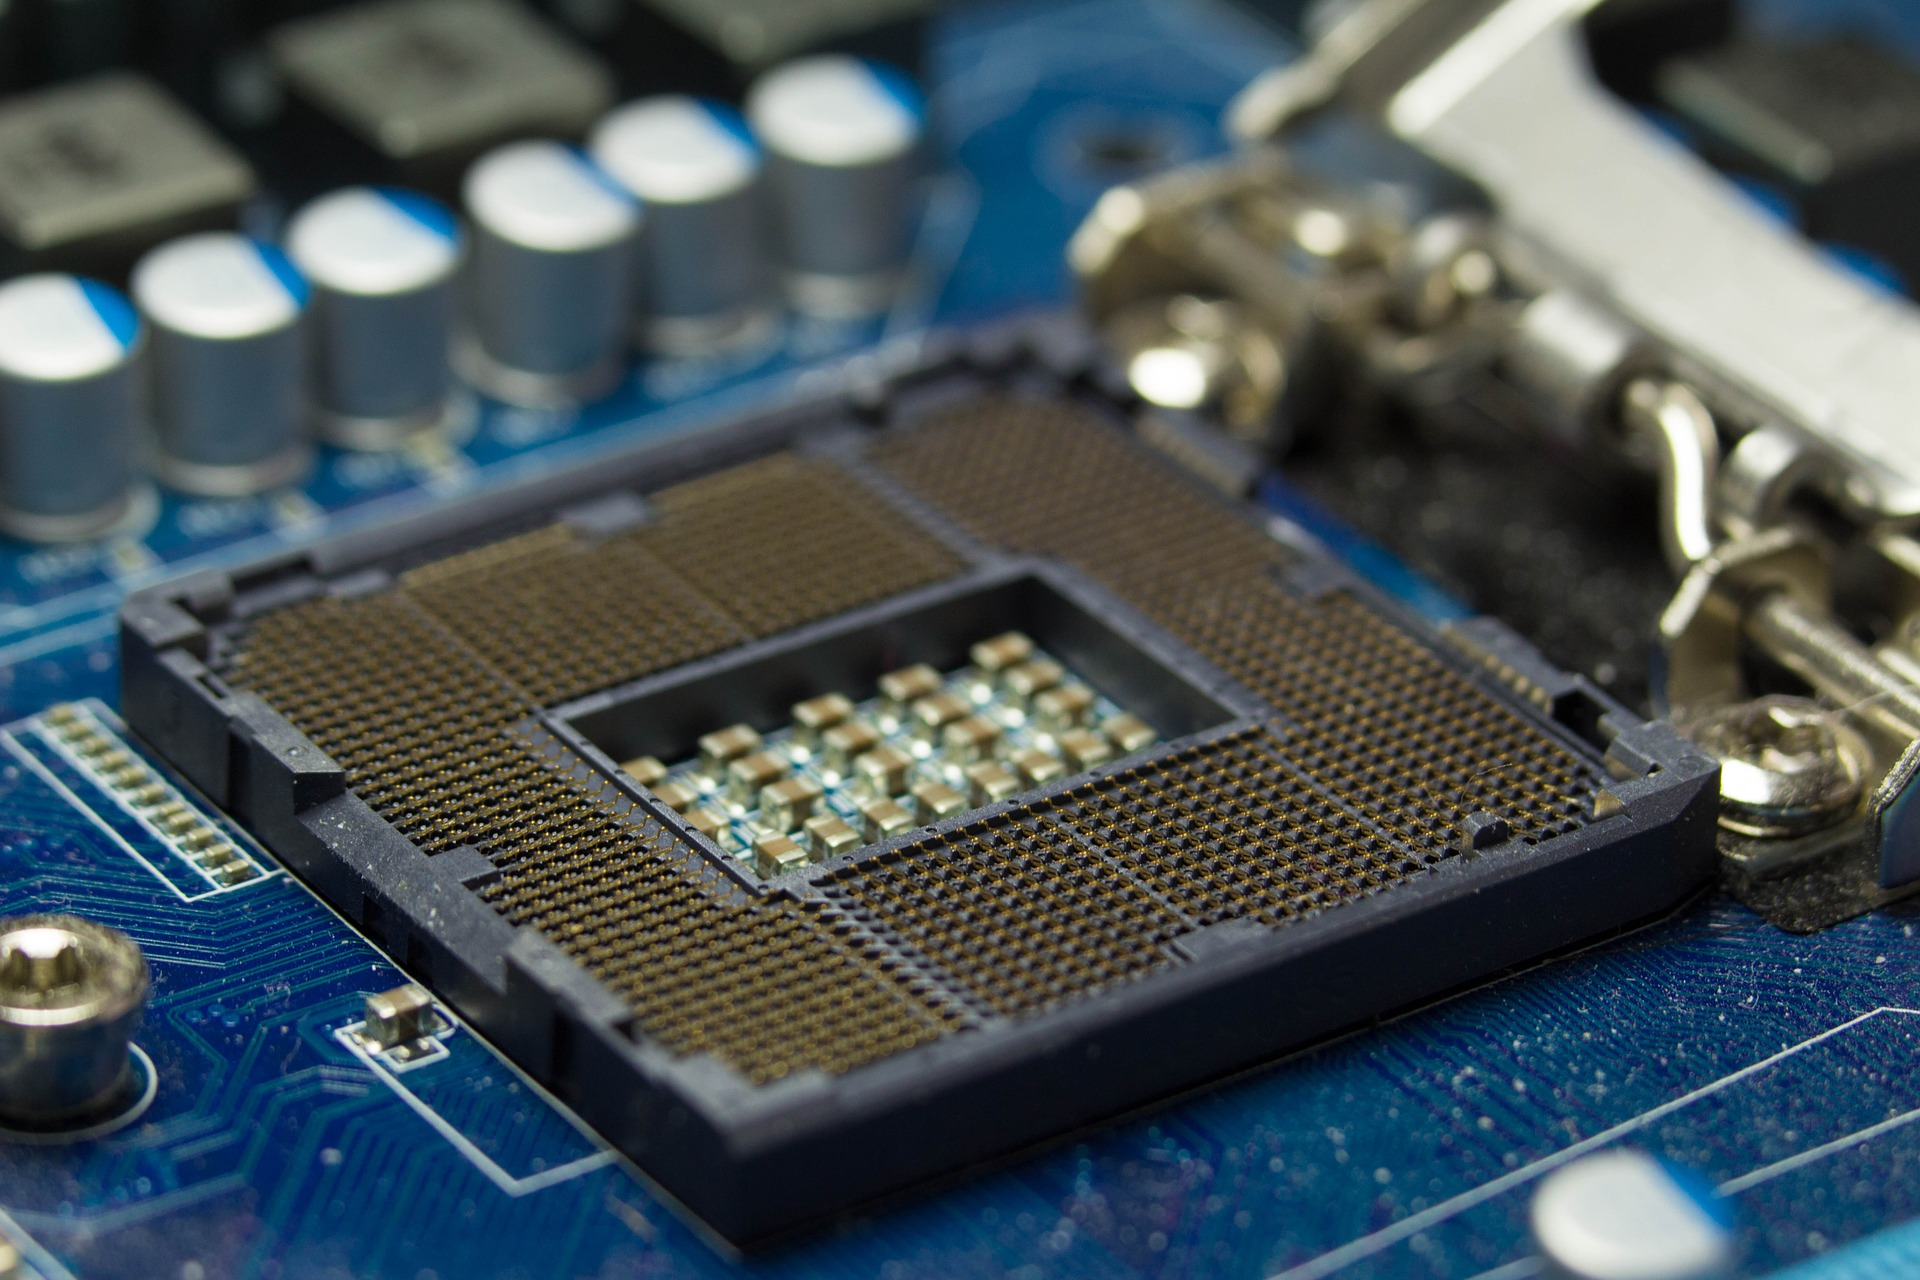
\includegraphics[height=3cm]{pictures/chip.jpg}
    \end{figure}
\end{nframe}

%%%%%%%%%%%%%%%%%%%%%%%%%%%%%%%%%%%%%%%%%%%%%%%%%%%%%%%%%%%%%%%%%%%%%%%%%%%%%%%%%%%%%%%%%%%%%%%%%%%%%%%%%%%%%%%%%%%%%%%%%%%%%%%%%%%

\section{The Cache Aware Roofline Model}

\begin{nframe}{The Cache Aware Roofline Model (CARM)}
  The Cache Aware Roofline Model~(CARM) simplifies this for you !
  
  \vspace{.5cm}
  \begin{itemize}
  \item \Large{What is the best you can get from the chip ? [Platform Model]}
    \vspace{.5cm}  
  \item \Large{Is it worth investing in code optimization ? [Application Model]}
  \end{itemize}
\end{nframe}

%%%%%%%%%%%%%%%%%%%%%%%%%%%%%%%%%%%%%%%%%%%%%%%%%%%%%%%%%%%%%%%%%%%%%%%%%%%%%%%%%%%%%%%%%%%%%%%%%%%%%%%%%%%%%%%%%%%%%%%%%%%%%%%%%%%

\begin{nframe}{Platform Model}
  Improvement over the Original Roofline Model~(ORM).

  \vspace{5mm}
  \begin{minipage}{.5\textwidth}
  Assumptions:

  \begin{itemize}
  \item The machine is bound whether by the memory unit or by the compute unit.
  \item Both unit are not dependent on each other.
  \end{itemize}
  \end{minipage}%
  \begin{minipage}{.5\textwidth}
  \begin{figure}
    \centering
    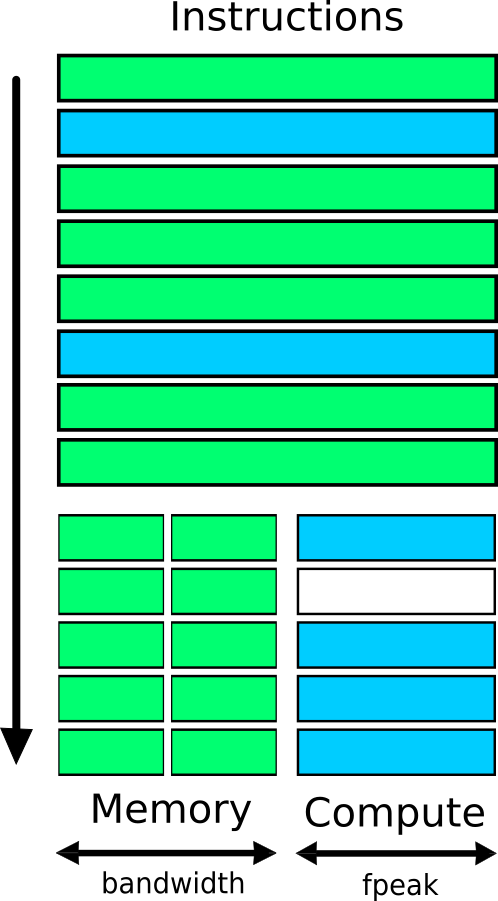
\includegraphics[width=\textwidth, height=.6\paperheight, keepaspectratio]{pictures/ORM_base.png}
  \end{figure}
  \end{minipage}
\end{nframe}

%%%%%%%%%%%%%%%%%%%%%%%%%%%%%%%%%%%%%%%%%%%%%%%%%%%%%%%%%%%%%%%%%%%%%%%%%%%%%%%%%%%%%%%%%%%%%%%%%%%%%%%%%%%%%%%%%%%%%%%%%%%%%%%%%%%

\begin{nframe}{Application Model}
  \vspace{1cm}
  \begin{equation}
    ddot = ddot + b[i] * c[i]
  \end{equation}

  \vspace{1cm}

  \begin{itemize}
  \item memory: ${b[i], c[i]} = 8+8 Bytes$
  \item compute: ${+,*} = 2 flops$
  \item operational intensity: $2^{-3} Flops/Bytes$
  \item performance: $Flops/Time$
  \end{itemize}
\end{nframe}

%%%%%%%%%%%%%%%%%%%%%%%%%%%%%%%%%%%%%%%%%%%%%%%%%%%%%%%%%%%%%%%%%%%%%%%%%%%%%%%%%%%%%%%%%%%%%%%%%%%%%%%%%%%%%%%%%%%%%%%%%%%%%%%%%%%

\begin{nframe}{ORM versus CARM}
  \begin{minipage}{.65\textwidth}
  \begin{figure}
    \centering
    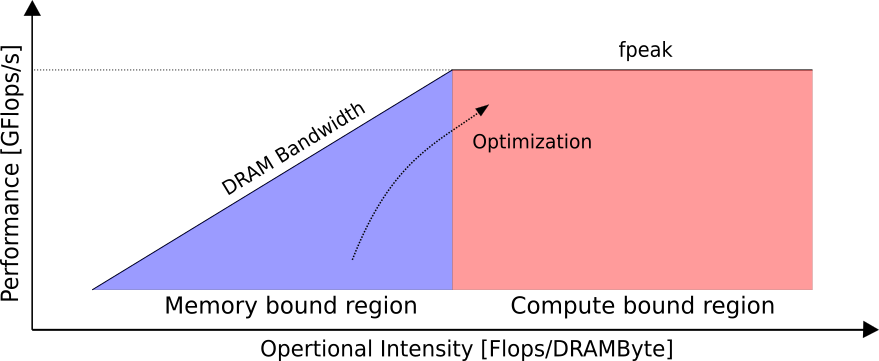
\includegraphics[width=\textwidth, height=.3\paperheight, keepaspectratio]{pictures/roofline_chart.png}
  \end{figure}
  \end{minipage}%
  \begin{minipage}{.3\textwidth}
    Bytes transferred from DRAM to last level cache
  \end{minipage}

  \vspace{5mm}
  \begin{minipage}{.65\textwidth}
  \begin{figure}
    \centering
    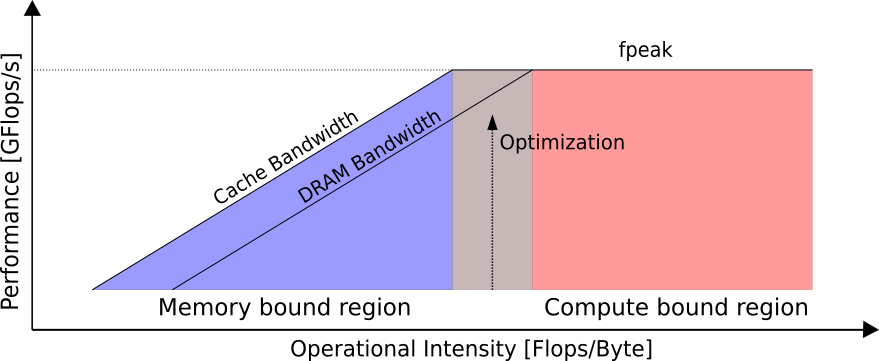
\includegraphics[width=\textwidth, height=.3\paperheight, keepaspectratio]{pictures/CARM_chart.png}
  \end{figure}
  \end{minipage}%
  \begin{minipage}{.3\textwidth}
    Bytes issued from Cores.
  \end{minipage}
\end{nframe}

%%%%%%%%%%%%%%%%%%%%%%%%%%%%%%%%%%%%%%%%%%%%%%%%%%%%%%%%%%%%%%%%%%%%%%%%%%%%%%%%%%%%%%%%%%%%%%%%%%%%%%%%%%%%%%%%%%%%%%%%%%%%%%%%%%%

\section{Tool and Validation}

\begin{nframe}{A Tool to Build and Validate the Model}
  \begin{block}{Build Model from Portable Blocks}
    \begin{itemize}
    \item Hwloc gives the machine informations: cache structure and attributes, cores.
    \item The compiler gives architecture type and let us select the best instruction set.
    \end{itemize}
  \end{block}

  \begin{block}{Micro-Benchmark Each Unit}
    \begin{itemize}
    \item Bandwidth benchmark each cache level, and several stream types: Load, Store, 2Loads/Store.
    \item Floating Point peak benchmark: MUL, ADD, MAD, FMA.
    \item Micro Benchmarks of several arithmetic intensities for validation.
    \end{itemize}
  \end{block}
\end{nframe}

\begin{nframe}{A Tool for Non Experts}
  \begin{block}{Easy steps}
    \begin{itemize}
    \item Build the model for the target platform.
    \item Collect CARM metrics from your application with our library (Hardware counters: PAPI).
    \item Plot this on a chart and get insights on your application.
    \end{itemize}
  \end{block}

  \begin{block}{Quick Glance if the Model is Wrong}
    \begin{itemize}
    \item Validation matches model ?
    \item Micro-Benchmarks matches theoretical throughput ?
    \end{itemize}
  \end{block}
\end{nframe}

\begin{nframe}{Tool Output}
  \begin{figure}
    \centering
    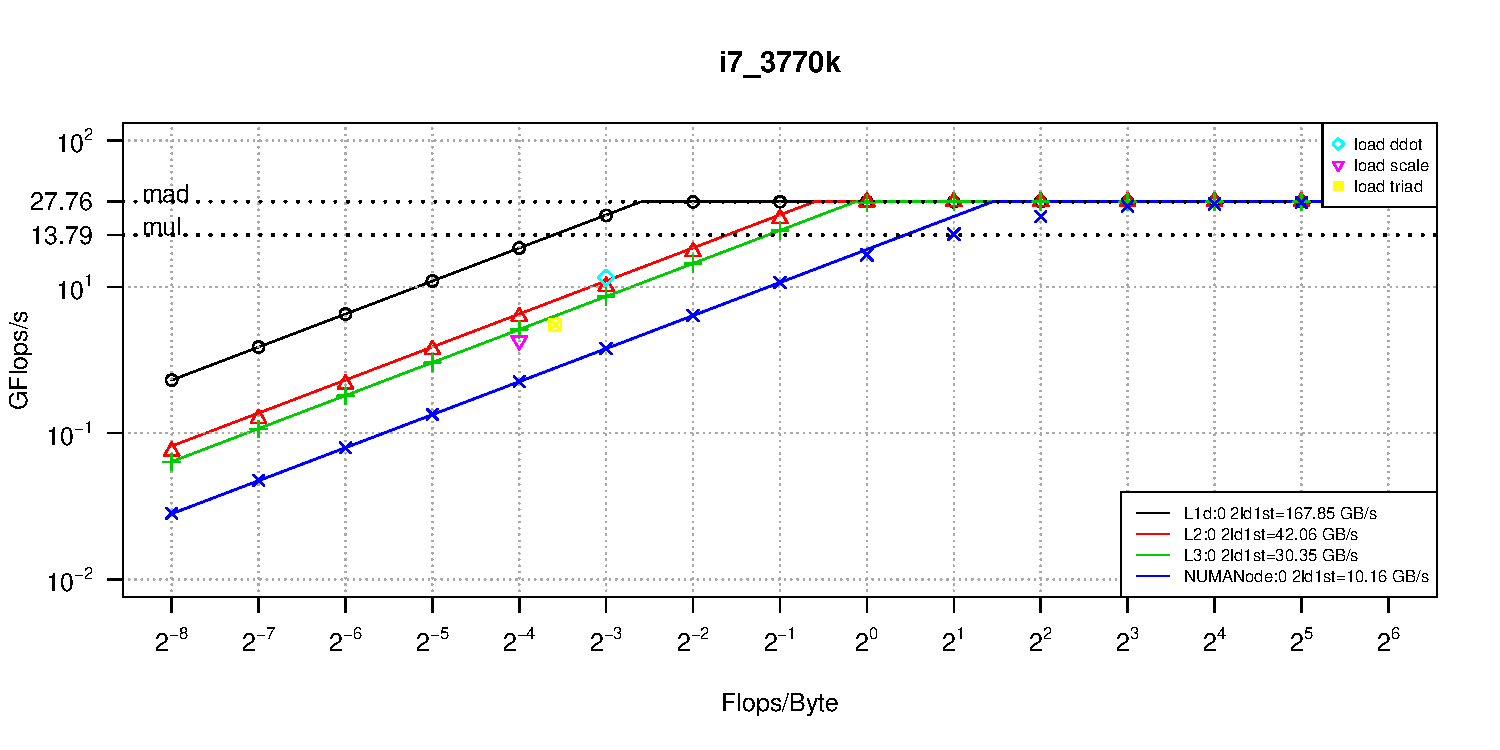
\includegraphics[width=\textwidth, height=.6\paperheight, keepaspectratio]{pictures/CARM_i7_3770k.pdf}
  \end{figure}  
\end{nframe}
%%%%%%%%%%%%%%%%%%%%%%%%%%%%%%%%%%%%%%%%%%%%%%%%%%%%%%%%%%%%%%%%%%%%%%%%%%%%%%%%%%%%%%%%%%%%%%%%%%%%%%%%%%%%%%%%%%%%%%%%%%%%%%%%%%%

\section{Conclusion \& Future Work}

\begin{frame}
  \begin{block}{Conclusion}
    We provide a Tool to build the CARM and model applications.

    It is portable and easy to use. It reaches near theoretical architecture throughput.
  \end{block}
  \begin{block}{Future Work}
    The CARM gives insight over Caches (i.e temporal locality).

    We will use it to model system heteogeneous memory, and give insights on data locality.
    
  \end{block}
\end{frame}
    

\begin{frame}
  \vspace{1cm}
  \begin{minipage}[t][.8\textheight]{\textwidth}
  \vspace{2.5cm}
  \centering
  {\LARGE{Thank you !}}

  \vfill
  \small{\href{https://github.com/NicolasDenoyelle/LARM-Locality-Aware-Roofline-Model-}{https://github.com/NicolasDenoyelle/LARM-Locality-Aware-Roofline-Model-}}
  \end{minipage}
\end{frame}




% Closing slide
\setbeamertemplate{headline}{}
\setbeamertemplate{footline}{}
\begin{frame}
   \begin{figure}
   
\includegraphics[height=1.5cm]{./logos/cost-logo.png}%
   \hspace{2cm}%
   
\includegraphics[height=1.5cm]{./logos/nesus-logo-01.png}  \\
   \end{figure}
  \titlepage
\end{frame}

\end{document}
